\section{Description of the user interface}\label{interface} 
The graphical user interface is very easy to use. An example is given in Figure~\ref{ui} (p. \pageref{ui}) of how the interface appears. 

\begin{figure}
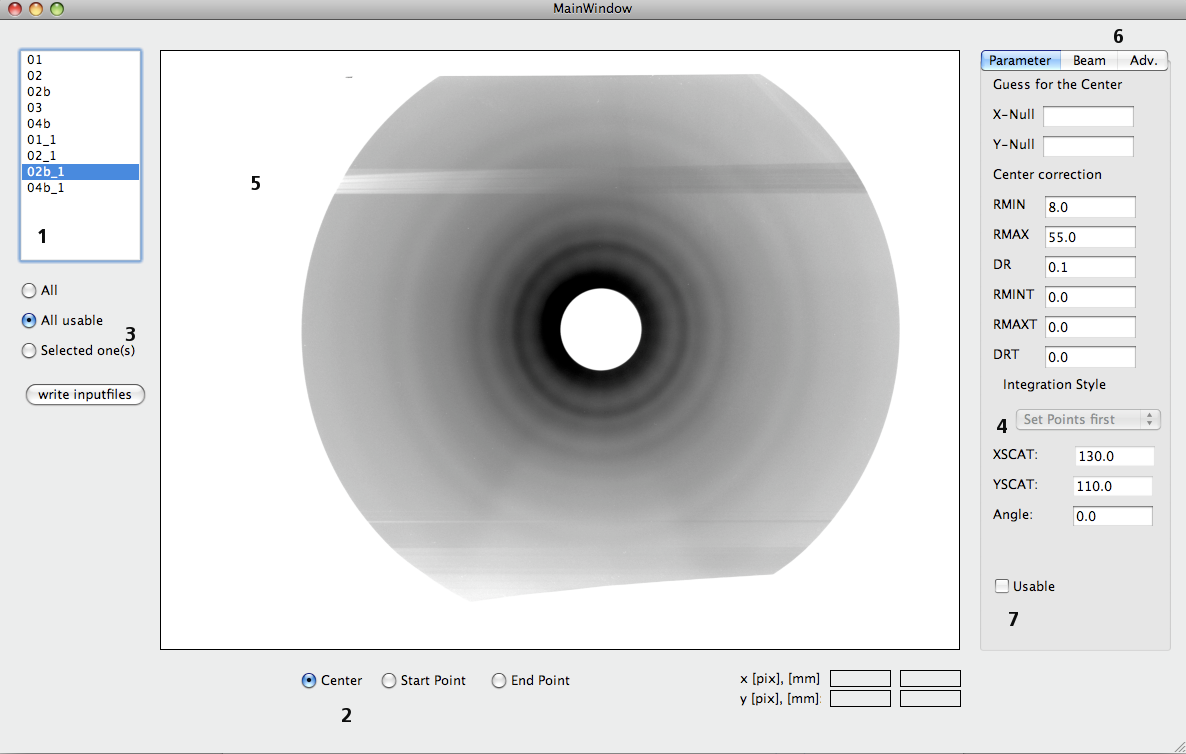
\includegraphics[width=20cm, angle=90]{ui.png}
\caption{Typical screenshot of the user interface. (1) The itemlist (listWidget), (2) Radiobuttons for selecting points, (3) Radiobuttons for selecting which input files to write out, (4) drop-down menu for selecting data reduction style, (5) main graphic, (6) tabs to set more parameters and (7) the Usable checkbox. }
\label{ui} 
\end{figure} 

\subsection{Input}
The program can deal with all kind of image formats. It was tested with .tif files but should work with all other formats, as long as they are supported by Qt. \\
The the images can be opened with the OpenFile menu. \\
The following should be considered:
\begin{enumerate}
\item The program assumes that the data files (.img) are in the same directory then the image files (.tif). 
\item The PIMAG executable must be in the same directory then the .tif and .img files. Otherwise the data reduction (see later) will not work. 
\end{enumerate}

\subsection{Workflow}
A complete workflow is described in Figure~\ref{workflow} (p. \pageref{workflow}). The workflow describes one way to work with the program. Theoretically it is possible to go back at any point of the diagram. 

\begin{figure}
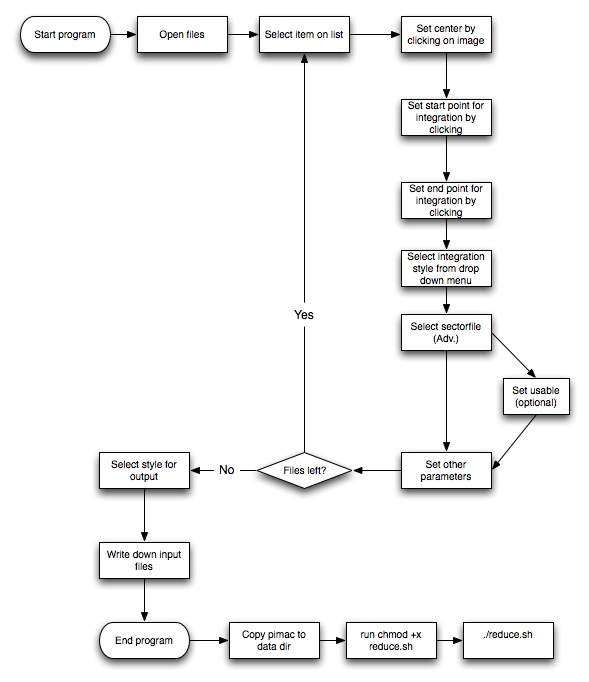
\includegraphics[width=12cm]{diagram}
\caption{Workflow of the program. The "set usable"-step is optional, depending on the way the input files are written out later. If you decide to write out input files for every image, it is not necessary to set.  }
\label{workflow} 
\end{figure} 
The first click on the graphic sets the approximetly center, the second click sets the start point and the third click sets the endpoint for the integration and an angle. This is also indicated by the radiobuttons (See Figure~\ref{ui} (p. \pageref{ui}). The angle is calculated depending on the selected integration mode.

\subsubsection{Selection integration mode}
There are several integration modes available: 
\begin{itemize}
\item [Whole area] This means that a circle with the center and radius determined above will be used for integration. If the measurement was good and there are no shadows on the plate, this is the best choice. 
\item[Top] The 'Top' half is taken for integration. The angle is determined by the endpoint relative to the y-axis (the center sets the zero point of the y axis). An example is given in Figure~\ref{modetop} (p. \pageref{modetop}).
\item [Down] The button half is taken for integration. Same as above, see example is given in Figure~\ref{modedown} (p. \pageref{modedown}).
\item [Top-Down] The 'Top' and 'Down' sectors are taken for integration. The angle is determined in the same way as above. An example is given in Figure~\ref{modetopdown} (p. \pageref{modetopdown}).
\item [Right]The right-hand side is taken for integration. The angle is the endpoint relative to the x-axis (the center is zero). An example is given in  Figure~\ref{moderight} (p. \pageref{moderight}).
\item [Left] Same as Right, but for the left side. See Figure~\ref{modeleft} (p. \pageref{modeleft}).
\item [Right-Left] The right- and left-hand sides are both taken into account. See Figure~\ref{moderightleft} (p. \pageref{moderightleft}).
\end{itemize}

\begin{figure}
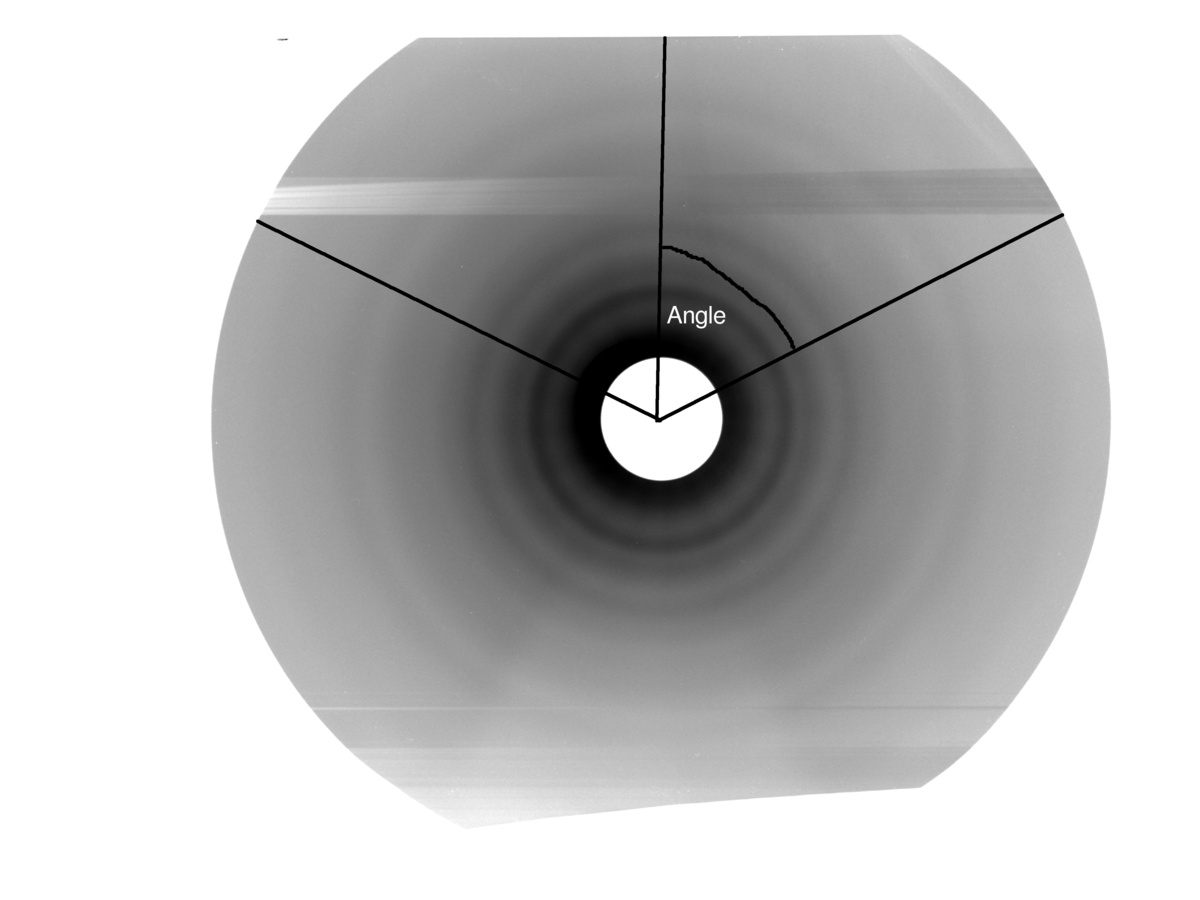
\includegraphics[width=12cm]{top.jpg}
\caption{Used sectors for mode \textit{Top}. }
\label{modetop} 
\end{figure} 

\begin{figure}
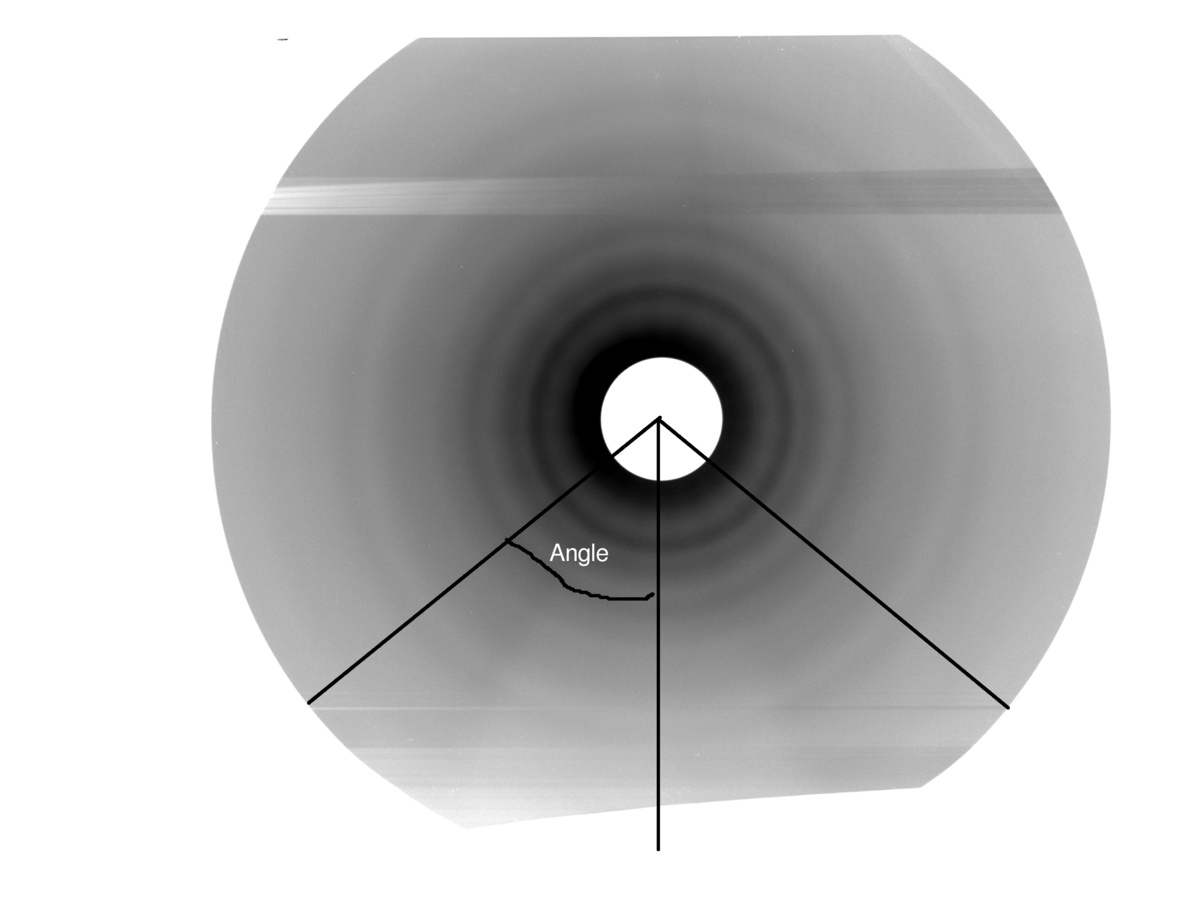
\includegraphics[width=12cm]{down.jpg}
\caption{Used sectors for mode \textit{Down}. }
\label{modedown} 
\end{figure} 

\begin{figure}
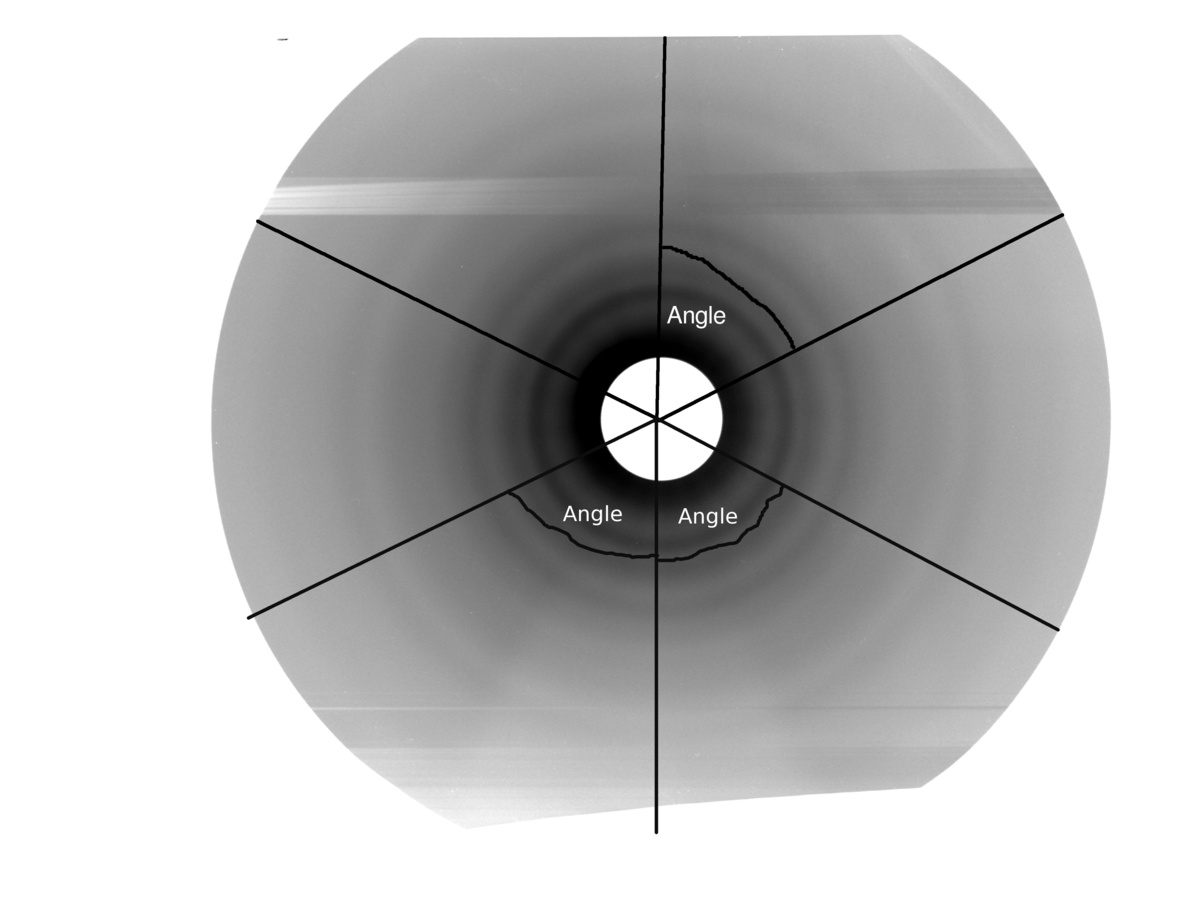
\includegraphics[width=12cm]{topdown.jpg}
\caption{Used sectors for mode \textit{Top-Down}. }
\label{modetopdown} 
\end{figure} 





\begin{figure}
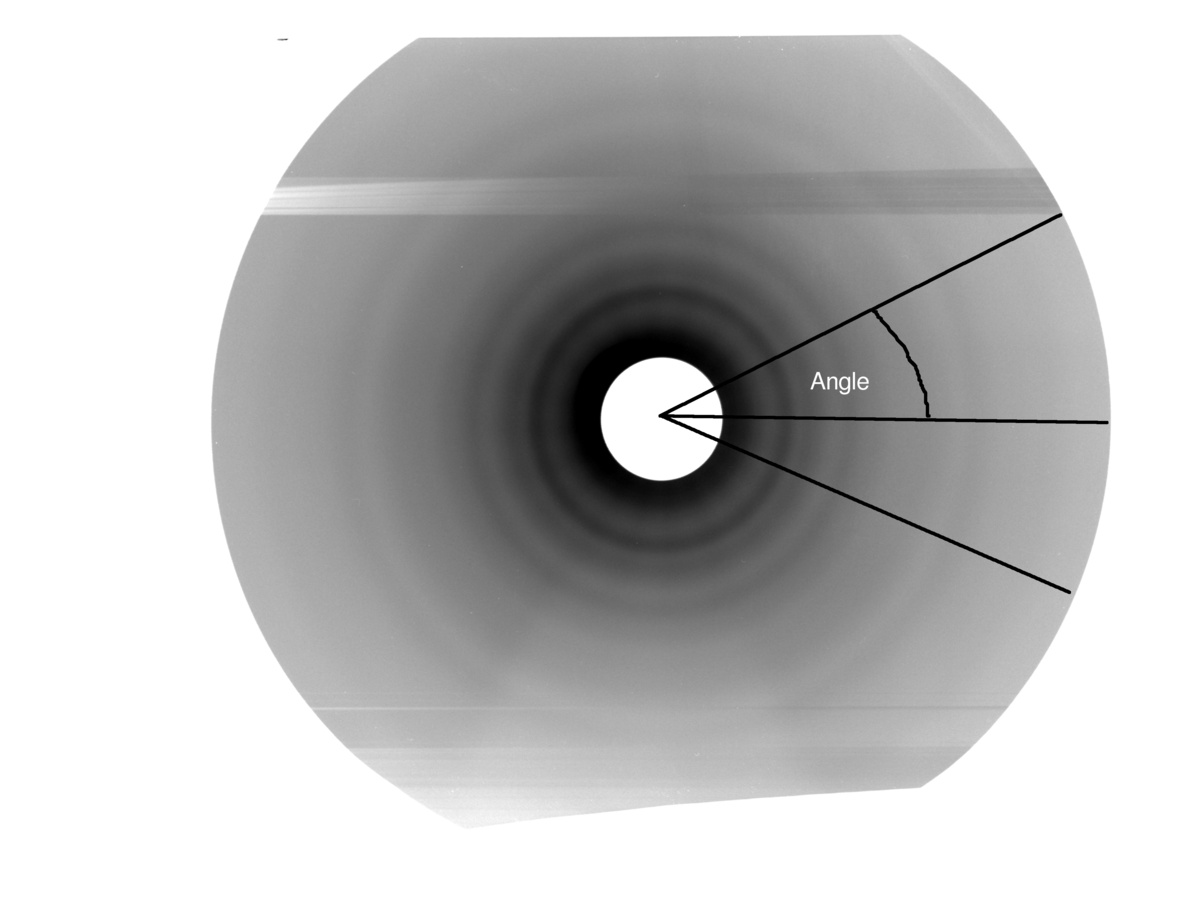
\includegraphics[width=12cm]{right.jpg}
\caption{Used sectors for mode \textit{Right}. }
\label{moderight} 
\end{figure} 

\begin{figure}
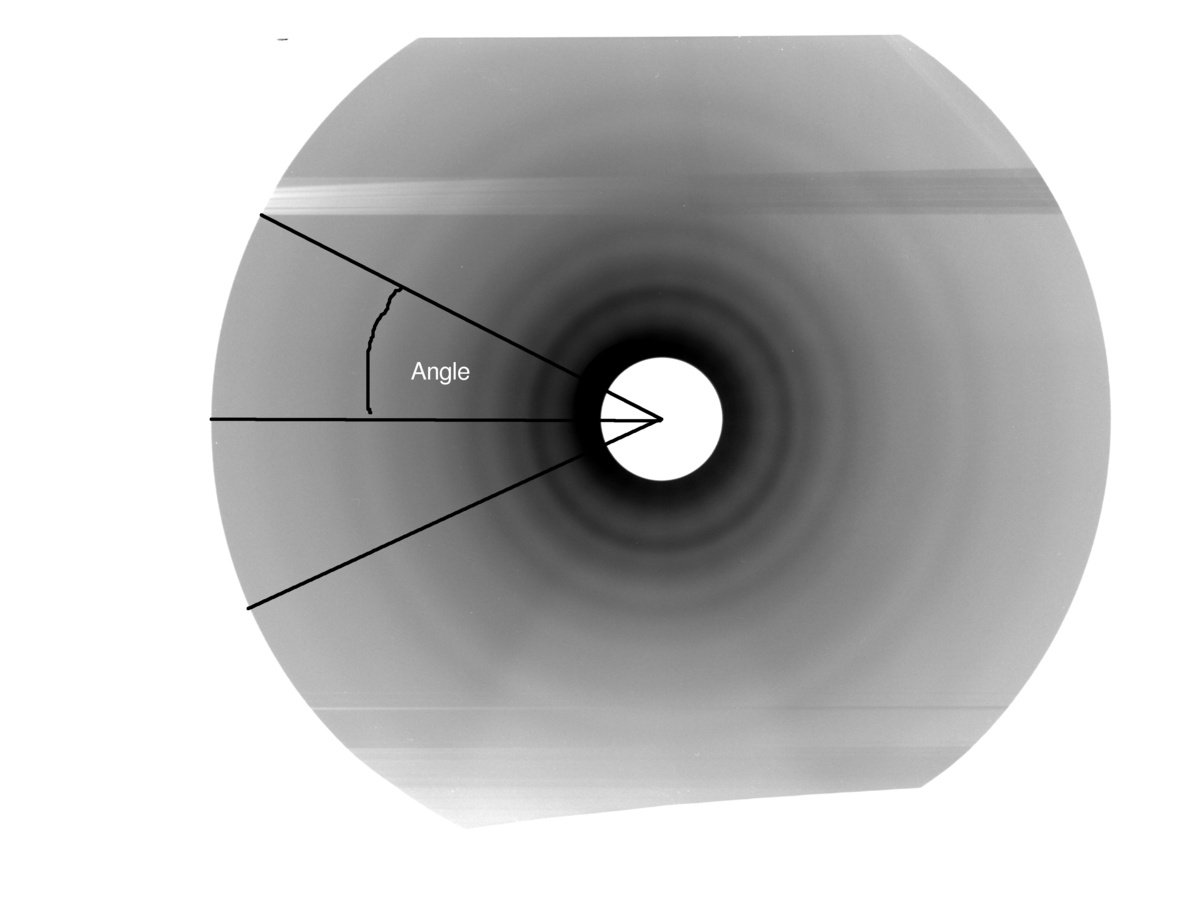
\includegraphics[width=12cm]{left.jpg}
\caption{Used sectors for mode \textit{Left}. }
\label{modeleft} 
\end{figure} 

\begin{figure}
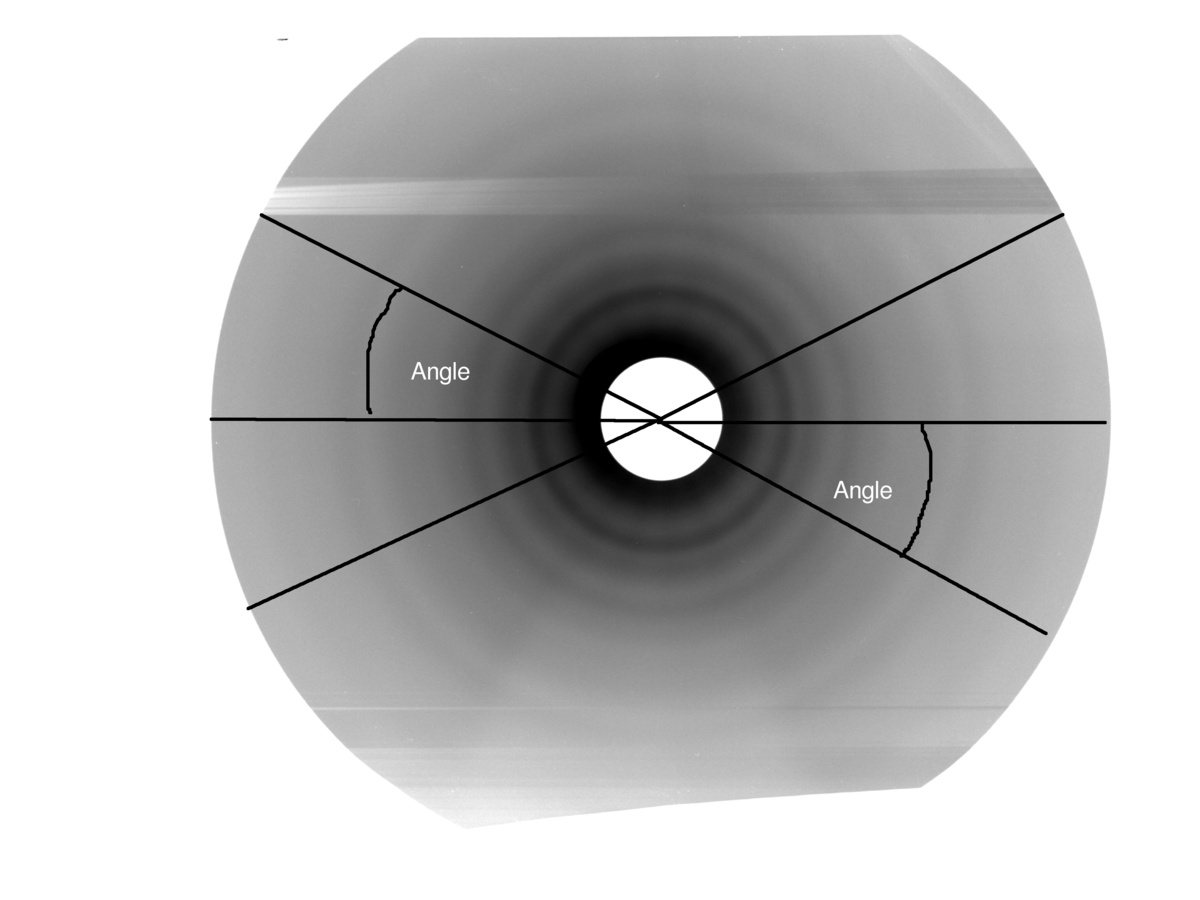
\includegraphics[width=12cm]{rightleft.jpg}
\caption{Used sectors for mode \textit{Right-Left}. }
\label{moderightleft} 
\end{figure} 
  
\subsection{Output}
The program has three modes to write out input files for PIMAG. For all images imported, for all images selected in the list or for all images flagged as usable. \\
For every image one .txt file is written out to the same directory as the image files. \\
In the end a bash-script is written to reduce.sh that can be used for data reduction. Notice that it must be executable (chmod +x) to execute it. Assuming the .tif and .img files are in /home/geduser/mydata/, the following has to be done: \\

\begin{lstlisting}
cd /home/geduser/mydata/
chmod +x reduce.sh
./reduce.sh 
\end{lstlisting}

The last command starts the data reduction. The script creates (or overwrites!) the following files, assuming that \$filename was the name of the .tif file, without the .tif.  

\begin{itemize}
\item [\$filename.curv] This file is used for further processing of the data. 
\item [\$filename.plot] This file is used for plotting, a free program like xmgr \cite{xmgr} or GNUPLOT \cite{gnuplot} can be used. 
\item [\$filename.info] This file contains detailed information about the data reduction process.
\end{itemize}




